\documentclass[../em.tex]{subfiles}
\graphicspath{{\subfix{../figures/}}}
\begin{document}
\chapter{Electric Circuits}
\section{Electric Current}
Current is the rate at which charge passes through a cross-sectional area of a wire.
\[I=\mathrm{d}q/\mathrm{d}t \implies q = \int I \mathrm{d}t\]
Current within a conductor consists charge carriers traveling through the conductor with an average drift velocity.
\[I=nqv_D A\]
Electric charge moves in a circuit in response to an electron potential difference, sometimes referred to as electromotive force, or emf ($\epsilon$)

Current density if the flow of charge per unit area.
\[I=\int{\vec{J}\cdot\mathrm{d}\vec{A}} \implies I = JA\]
Current density is related to the motion of the charge carriers within a conductor and is a vector quantity.
\[J=nqv_D\]
A potential difference across a conductor creates an electric field within the conductor that is proportional to the resistivity and the current density.
\[\vec{E}=\rho \vec{J}\]
If a function of current density is given, the total current can be determined by integrating the density over the area.
\[I=\int \vec{J(r)}\cdot\mathrm{d}\vec{A}\]
Although current is a scalr quantity, it does have direction.
\begin{itemize}
    \item The direction of conventional current is chosen to be the direction in which positive charge would move.
    \item In common circuits, the current is actually due to the movement of electrons.
\end{itemize}

\begin{example}
    A long conducting cylinder has radius $R$, and carries a current to the left. The current density varies with distance 
    $r$ from the cylinder's central axis according to the equation $J=kr^2$, where $r\leq R$ and $k$ is a positive constant. Derive an expression
    for the total current in the cylinder.

    \begin{align*}
        I=\int\vec{J}(r)\cdot\mathrm{d}\vec{A} \\
        = \int (kr^2)(2\pi r\mathrm{d}r)
        = \frac{\pi k}{2}R^4
    \end{align*}
\end{example}

\ex Two different wires are both carrying uniform currents. Wire 1 has a cross-sectional area $A_1$, resistivity $\rho_1$ and a current $I_1$. Wire 2 has a cross-sectional area $2A_1$, resistivity $3\rho_1$,
and a current $2I_1$. What is the ratio $E_2:E_1$ of the electric magnitude in wire 2 to the electric field magnitude in wire 1?

\ex Two conducting wires, Wire X and Wire Y, have the same length and cross-sectional area but are made of different materials. The charge carriers in two wires are electrons, and have densities in wires X and Y of 
$4.22\times 10^{22}$ cm$^{-3}$ and $8.0\times 10^{22}$ cm$^{-3}$ respectively. Wire Y has three times the current of Wire X. What is the ratio $\frac{v_y}{v_x}$ of the average drift velocity $v_Y$ in wire Y to the average drift velocity $v_X$ in wire X?

\section{Simple Circuits}
A circuit is composed of electrical loops, which can include wires, batteries, resistors, 
lightbulbs, capacitors, inductors, switches, ammeters, and voltmeters.

A closed electrical loop is a closed path through which charges may flow.
\begin{itemize}
    \item A closed circuit is one in which charges would be able to flow.
    \item An open circuit is one in which charges would not be able to flow.
    \item A short circuit is one which charges would be able to flow with no change in potential difference.
\end{itemize}

Circuit schematics are representations used to describe and analyze electric circuits.
\begin{itemize}
    \item The properties of an electric current are dependent on the physical arrangement of its constituent elements.
\end{itemize}
Circuit elements have common symbols that are used to create schematic diagrams.
\begin{itemize}
    \item If an element is variable, then the element is indicated by a diagonal strikethrough arrow across the symbol.
\end{itemize}
\begin{center}
    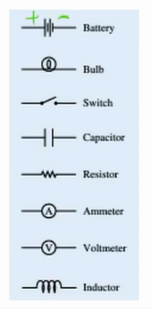
\includegraphics[width=0.2\textwidth]{appc111.PNG}
\end{center}

\ex 
\begin{center}
    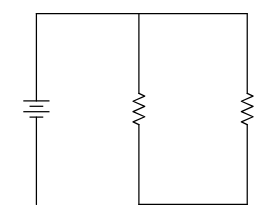
\includegraphics[width=0.5\textwidth]{11.3.PNG}
\end{center}
The figure shows a battery connected to two resistors. Is there current in the resistors? What evidence or reasoning supports the claim?

\pagebreak
\section{Ohm's Law and Electrical Power}
\begin{itemize}
    \item Resistance is a measure of the degree to which an object opposes the movement of electrical charge.
    \item It is proportional to its resistivity and length and is inversely proportional to its cross-sectional area.
    \[R=\frac{\rho l}{A}\]
    \item This assumes the resistivity to be uniform.
    
    \item If the resistivity is not uniform, meaning it varies along the length, use:
    \[R=\int{\frac{\rho(l)}{A}}\mathrm{d}l\]

    \item Ohm's Law relates current, resistance, and potential difference across a conductive element of current.
    \[I=\frac{\Delta V}{R}\implies V = IR\]

    \item The resistivity of an ohmic material is constant regardless of temperature.
    
    \item The resistance of an ohmic circuit element can be determined from the slope of a graph of the current in the element as a function of the potential difference across the element.
    \item The rate at which energy is transferred, converted or dissipated by a circuit element depends on the current in the element and the electrical potential difference across it.
    \item The brightness of a lightbulb increases with power, so power can be used to qualitatively predict the brightness of lightbulbs in a circuit.
\end{itemize}

\begin{example}
    Long cables can sometimes act like antennas, picking up electronic noise, which are signals from other equipment and applicances. Coaxial cables are used for many applications 
    that require this noise to be eliminated. For example, they can be found in the home in cable TV connections or other audiovisual connections. Coaxial cables consist of an inner conductor 
    of radius $r_i$ surrounded by a second, outer concentric conductor with radius $r_0$. The space between the two is normally filled with an insulator such as polyethylene plastic.
    A small amount of radial leakage current occurs between the two conductors. Determine the resistance of a coaxial cable of length $L$.

    \[ R=\frac{\rho L}{A}\implies \dd R = \frac{\rho}{A}\dd r \implies R = \frac{P}{2\pi L}\int_{r_i}^{r_o}\frac{1}{r}\dd r \]

    Solving this results in $\frac{P}{2\pi L}\ln\left(\frac{r_0}{r_i}\right)$
\end{example}

\ex A wire has a length of 0.5 m, a circular cross section of radius $2.0\times 10^{-4}$ m, and a resistance of $2.5\Omega$. What is the resistivity of the material used to make the wire?

\ex A $10\Omega$ resistor has a current that varies with time $t$ according to the equation $I(t)=I_0e^{-\alpha t}$, where $I_0 = 4$A and $\alpha = 2$ s$^{-1}$. What is the total energy dissipated in the resistor between $t=0$ and a long time later?

\section{Compound Direct Current Circuits}
Circuit elements may be connected in series and/or parallel.

A series connection is one in which any charge passing through one circuit element must proceed through all elements in that connection and has no other path available.

The current in each series circuit element is the same.

A parallel connection is one in which chargesm ay pass through one of two or more paths.

Across each path, the potential difference is the same.

Ideal batteries and wires have negligible internal resistance.

If the battery is not ideal, then it has an internal resistance.
\[\Delta V_{\text{Terminal}}=\epsilon - IR \]
Ammeters are used to measure current at a specific point in a circuit. It must be connected in series in the circuit.

Voltmeters are used to measure the electric potential difference between two points in a circuit. They must be connected in parallel.

\begin{example}
    The figures below show parts of two circuits, each containing a battery of emf $\epsilon$ and internal resistance $r$. The current in each battery is 1 A, but the direction in one battery 
    is opposite to that in the other. If the potential differences across the batteries' terminals are 10 V and 20 V as shown, what are the value of $\epsilon$ and $r$?

    \begin{center}
        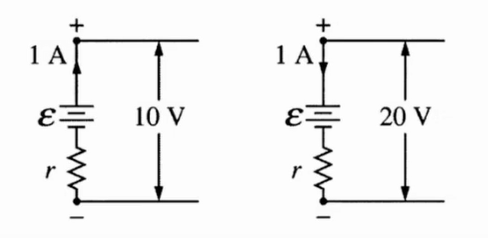
\includegraphics[width=0.5\textwidth]{11.4.PNG}
    \end{center}

    From the Kirchoff we have both $10=\epsilon-(1)r$ and $-20=-\epsilon+(1)r$.

    Solving this system of equations gives $\epsilon = 15$ V and $r = 5 \Omega$.   
\end{example}

\ex \begin{center}
    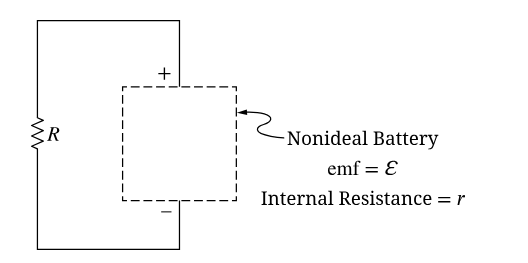
\includegraphics[width=0.5\textwidth]{11.4.1.PNG}
\end{center}
The figure shows a circuit with resistor of resistance $R$ connected to a nonideal battery. The battery has emf $\epsilon$ and an internal resistance $r$. What is the current generated by the battery?

\ex Two batteries have the same emf, but one battery is ideal while the other battery is nonideal. The batteries are connected to identical resistors. Does the resistor connected to the nonideal battery 
have the same or less current compared to the resistor connected to the ideal battery? What evidence or reasoning helps support this claim?

\pagebreak
\section{Kirchoff's Rules}
\begin{itemize}
    \item Kirchoff's Rules quantify how current flows through a circuit and how voltage varies around a loop in a circuit.
    \item Kirchoff's Loop Rule is a consequence of the conservation of energy.
    \begin{itemize}
        \item This is sometimes called Kirchoff's Voltage Law.
        \item It states that the sum of the potential differences across all circuit elements in a single closed loop must equal zero.
        \[\sum V = 0\]
    \end{itemize}
    \item Kirchoff's Junction Rule is a consequence of the conservation of charge.
    \begin{itemize}
        \item This is sometimes called Kirchoff's Current Law.
        \item It states the total amount of charge entering a junction per unit time must equal the total amount of charge exiting the junction per unit time.
        \[\sum I = 0\]
    \end{itemize}
\end{itemize}

\begin{example}
    In the circuit below, the emf's and the resistances have the values shown. The current $I$ in the circuit is 2 amperes. The potential difference between points $X$ and $Y$ are?

    \begin{center}
        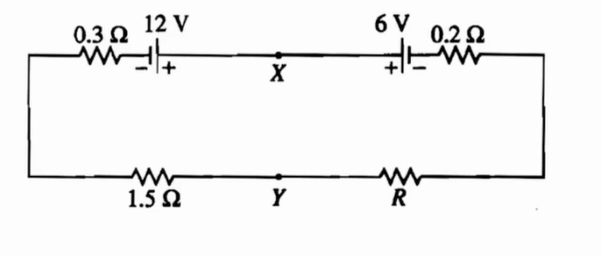
\includegraphics[width=0.5\textwidth]{11.5.PNG}
    \end{center}

    The voltage equation for this circuit is $12$V - $6V$ - $(0.2)(2)$ - $2R$ - $(1.5)(2)$ - $0.3(2) = 0$. Solving this gives $R=1$.

    Plugging this back in we get that $6+(0.2)(2)+(1)(2)=8.4$ V.
\end{example}

\begin{example}
    Two resistors of resistances $R$ and $12\Omega$ are connected to a battery of emf 18 V, as shown in the figure below. The battery has an internal resistance of $r$. The current in the battery 
    is 1.5 A, and the current in the $12\Omega$ resistor is 1.0 A. What is the resistance $R$?

    \begin{center}
        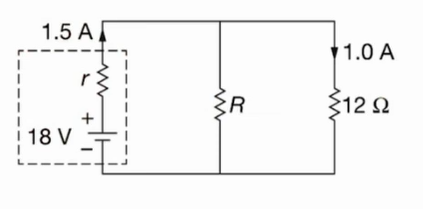
\includegraphics[width=0.5\textwidth]{11.5.1.PNG}
    \end{center}

    We have two equations, the first being $18V-1.5R-(1.0)(12)=0$ and $-18V+1.5R+0.5R=0$.

    Solving for $R$ we get that this is equal to $24\Omega$.
\end{example}

\pagebreak
\ex \begin{center}
    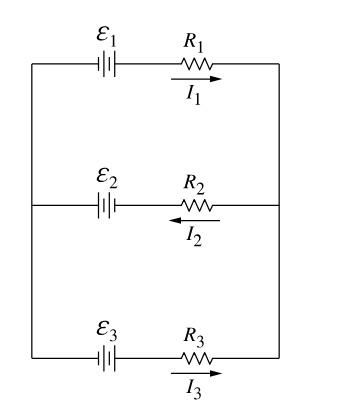
\includegraphics[width=0.5\textwidth]{11.5.2.PNG}
\end{center}
The figure shows a circuit with three batteries and three resistors with the emf of each battery and the resistance of each resistor as indicated. 
Write an equation that expresses a Kirchoff's loop rule for a portion of the circuit.

\ex \begin{center}
    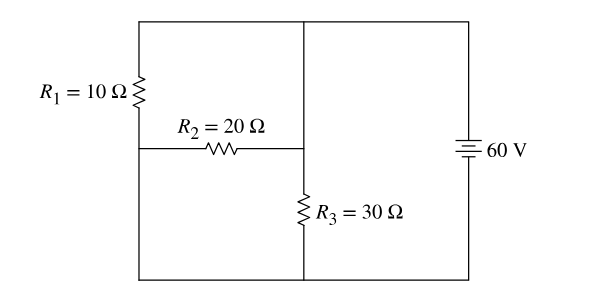
\includegraphics[width=0.5\textwidth]{11.5.3.PNG}
\end{center}
The figure shows three resistors connected to a battery, with the resistances and emf indicated. 
Rank the potential differences $\Delta V_1$, $\Delta V_2$, and $\Delta V_3$ across resistors $R_1$, $R_2$, and $R_3$, respectively?

\section{Resistor-Capacitor (RC) Circuits}
A collection of capacitors in a circuit may be analyzed as though it was a single capacitor with an equivalent capacitance $C_{ep}$.

As a result of conservation of charge, each of the capacitors in series must have the same magnitude of charge on each plate.

The charge on a capacitor or the current in a resistor in a RC circuit can be described by a 
fundamental differential equation derived from Kirchoff's loop rule.
\[ \epsilon = \frac{\dd q}{\dd t}R+\frac{q}{C} \]

The time constant ($\tau$) is a significant feature of an RC circuit.

The time constant of an RC circuit is a measure of how quickly the capacitor will charge or discharge and is defined as 
\[\tau = RC\]

\begin{example}
    A relaxation oscillator is used to control a pair of windshield wipers. The relaxation oscillator consists of a 10.00 mF capacitor and a 10.00 k$\Omega$ variable resistor known as a rheostat.
    A knob connected to the variable resistor allows the resistance to be adjusted from $0.00\Omega$ to $10.00$k$\Omega$. 

    The output of the capacitor is used to control a voltage-controlled switch. The switch is normally open, but when the output reaches 10.00 V, the switch closes, energizing an electric motor and discharging the capacitor. The motor 
    causes the windshield wipers to sweep once across the windshield and the capacitor begins to charge again. To what resistance should the rheostat be adjusted for the period of the wiper blades to be 10.00 seconds?

    We start with $\epsilon = [\frac{\dd q}{\dd t}+\frac{q}{c}]/R$.

    From this we have that $\dd t = \frac{\dd q}{\frac{\epsilon}{R}-\frac{q}{RC}}$.

    Solving for $R$ gives $R=\frac{-t}{C[\ln[1-\frac{V_D}{V}]]}=558.11 \Omega$.
\end{example}

\ex $N$ identical capacitors are placed in series with each other. What is the ratio of the equivalent capacitance of the series set to the capacitance of a single capactior?

\ex \begin{center}
    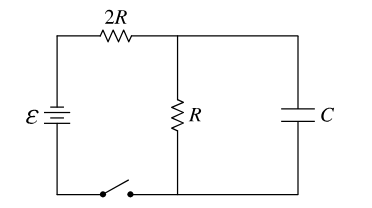
\includegraphics[width=0.5\textwidth]{11.6.1.PNG}
\end{center}
In the circuit shown in the figure, the switch has initially been opened for a long time. The switch is then closed. Immediately after the switch is closed, the current in resistor 2R is $I_i$.
A long time after the switch is closed, the current in the resistor 2R is $I_f$. What is the approximate value of the ratio $\frac{I_f}{I_I}$?

\end{document}